\documentclass{beamer}

\usepackage{graphicx}
\graphicspath{ {results} }

\begin{document}

    \begin{frame}{Background}
        \begin{itemize}\setlength\itemsep{15pt}
            \item {
                Microarrays measure the expression of thousands of genes simultaneously. 
            }
            \item {
                Microarray data is being used for early diagnosis of cancer.
            }
            \item {
                Researchers are struggling to extract meaningful information from so much data.
            }
            \item {
                We propose an application of machine learning to make diagnoses from microarray data.
            }
        \end{itemize}
    \end{frame}

    \begin{frame}{Procedure}
        \begin{itemize} \setlength\itemsep{15pt}
            \item {
                We will perform multi-class classification to diagnose samples
                as healthy or cancerous and determine what type of cancer.
            }
            \item {
                We will compare traditional ML (logistic regression with PCA) 
                and deep learning.
            }
            \item {
                We will compare different set of genes (as features) to determine which
                has more diagnostic power.
            }
        \end{itemize}
    \end{frame}
    
    \begin{frame}{Data}
        \begin{itemize} \setlength\itemsep{15pt}
            \item {
            }
        \end{itemize}
    \end{frame}

    \begin{frame}{Cross Validation Results}
        \begin{center}
            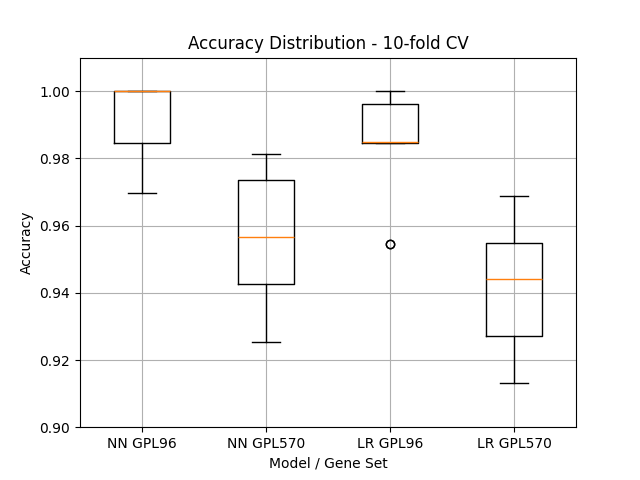
\includegraphics[scale=.63]{accdist.png}
            \vspace{15pt}
        \end{center}
    \end{frame}

    % put nn on the left
    \begin{frame}{Confusion Matrix - GPL96}
        \begin{center}
            \hspace{-70pt}
            \begin{minipage}{0.4\textwidth}
                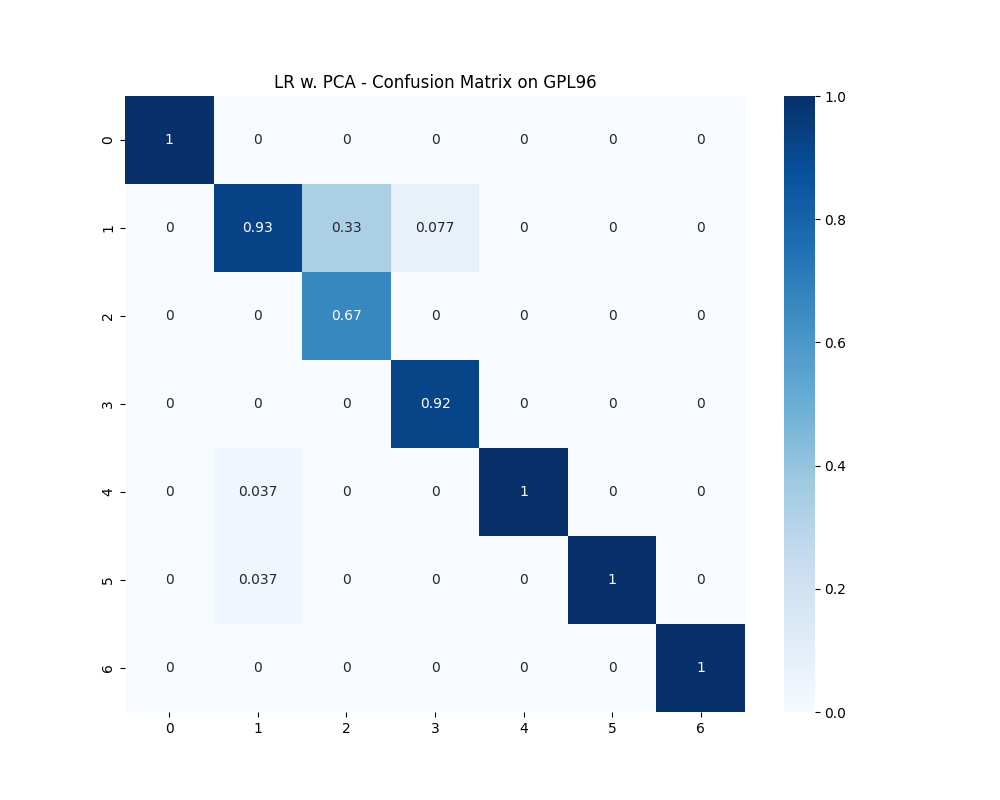
\includegraphics[scale=.3]{LRGPL96confusion.png}
            \end{minipage}
            \hspace{30pt}
            \begin{minipage}{0.4\textwidth}
                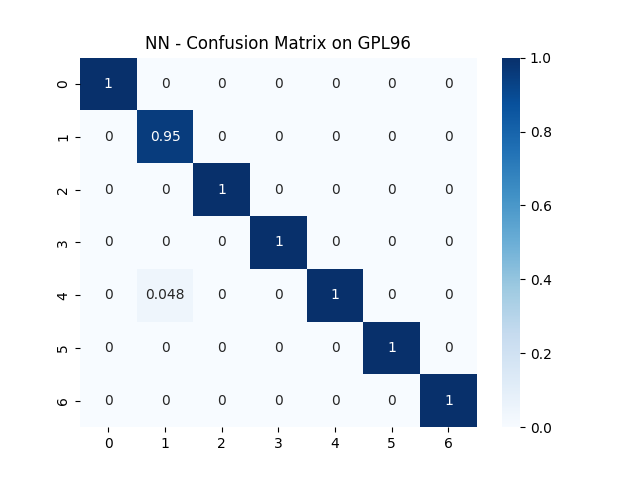
\includegraphics[scale=.3]{NNGPL96confusion.png}
            \end{minipage}
        \end{center}
    \end{frame}

    \begin{frame}{Confusion Matrix - GPL570}
        \begin{center}
            \hspace{-70pt}
            \begin{minipage}{0.4\textwidth}
                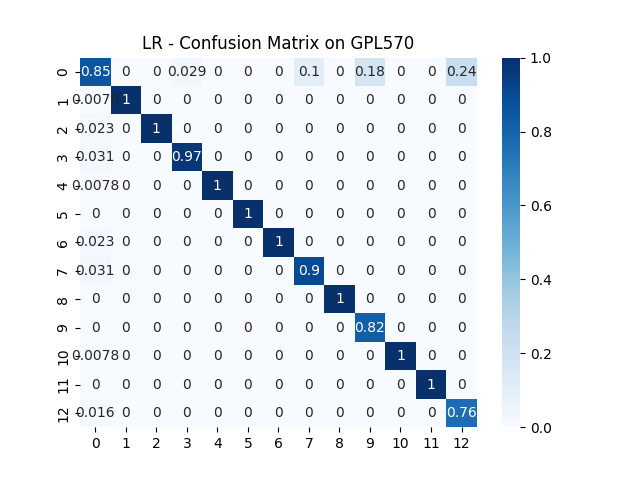
\includegraphics[scale=.3]{LRGPL570confusion.png}
            \end{minipage}
            \hspace{30pt}
            \begin{minipage}{0.4\textwidth}
                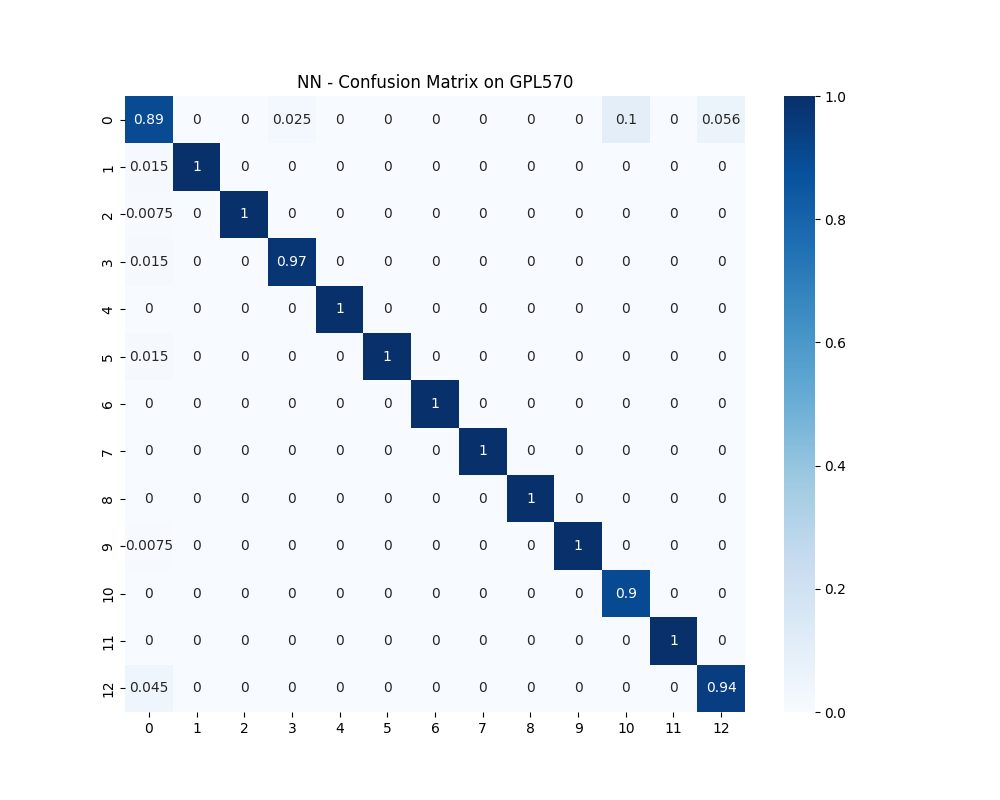
\includegraphics[scale=.3]{NNGPL570confusion.png}
            \end{minipage}
        \end{center}
    \end{frame}

    \begin{frame}{ROC Curve - GPL96}
        \begin{center}
            \hspace{-60pt}
            \begin{minipage}{0.4\textwidth}
                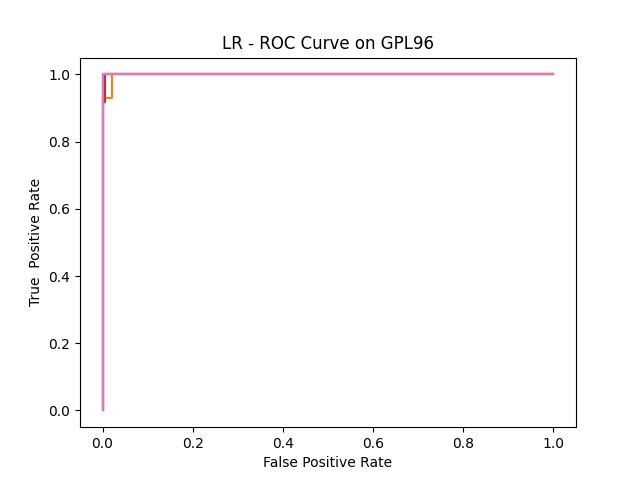
\includegraphics[scale=.4]{LRGPL96ROC.png}
            \end{minipage}
            \hspace{40pt}
            \begin{minipage}{0.4\textwidth}
                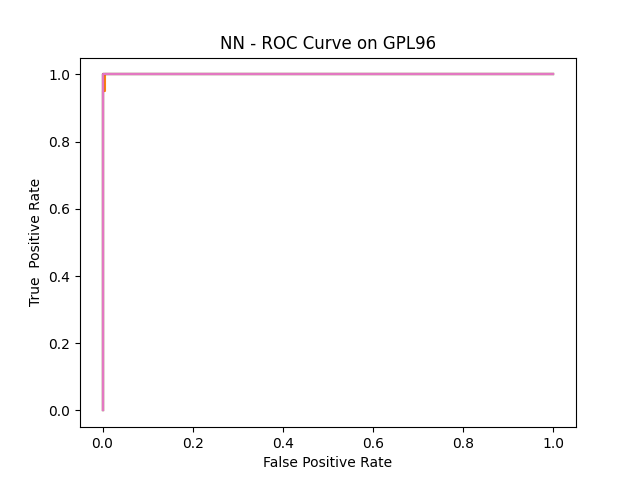
\includegraphics[scale=.4]{NNGPL96ROC.png}
            \end{minipage}
        \end{center}
    \end{frame}

    \begin{frame}{ROC Curve - GPL570}
        \begin{center}
            \hspace{-60pt}
            \begin{minipage}{0.4\textwidth}
                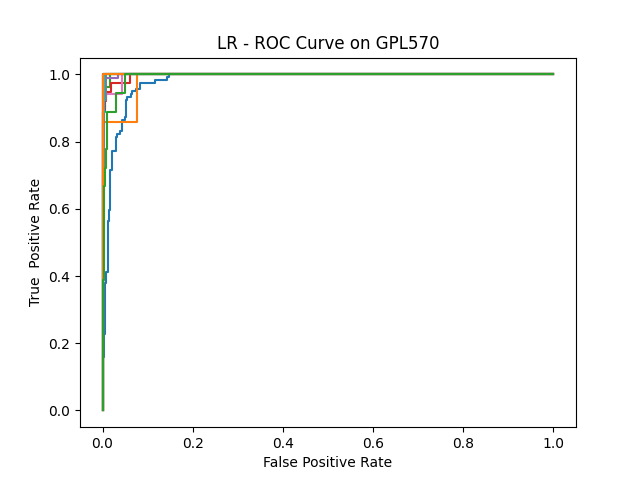
\includegraphics[scale=.4]{LRGPL570ROC.png}
            \end{minipage}
            \hspace{40pt}
            \begin{minipage}{0.4\textwidth}
                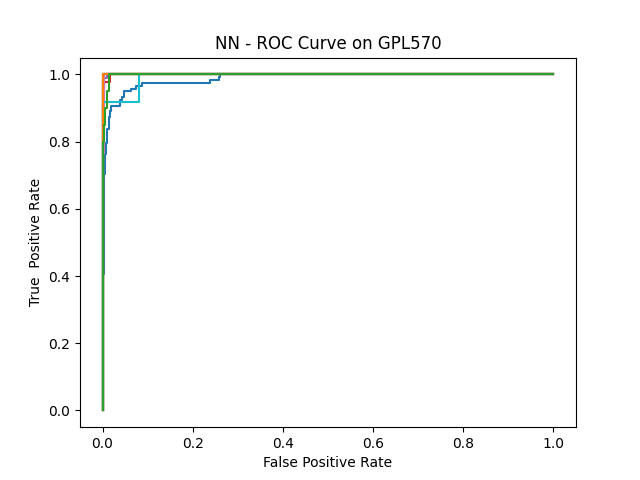
\includegraphics[scale=.4]{NNGPL570ROC.png}
            \end{minipage}
        \end{center}
    \end{frame}

    \begin{frame}{Open Questions and Next Steps}
        \begin{itemize} \setlength\itemsep{15pt}
            \item {
                If we restrict the GPL570 to the 7 classes present in GPL96,
                will performance improve? To address the information
                content of the gene sets, we need to 
                perform this experiment.
            }
            \item {
                ``Beautify'' plots by adding labels to each class (healthy, lung cancer, etc.).
            }
            \item {
                Draw conclusions and prepare a presentation.
            }
        \end{itemize}
    \end{frame}


\end{document}